\documentclass{beamer}

\usetheme{Boadilla}

\usepackage{listings}

\usepackage{hyperref}
\hypersetup{colorlinks=true}
\title{Udacity nanodegree overview}
\author{Kurbakov Dmytro}

\begin{document}
\begin{frame}
\titlepage
\end{frame}

\begin{frame}{Overview}
\tableofcontents
\end{frame}


\section{Nanodegree.. what does it mean?}

\begin{frame}
\begin{center}
\Huge Nanodegree.. what does it mean?
\end{center}
\end{frame}

\begin{frame}[fragile]{Definition}
A Udacity Nanodegree® Program is a unique online educational offering designed to bridge the gap between learning and career goals. (Udacity)
\newline
\newline
Set of the learning courses with a focus on the practical side (Kurbakov D.). 

\end{frame}

\begin{frame}[fragile]{Who is a teacher?}
Short answer: Partners with Udacity Full time employees.

Partners;
\begin{itemize}
\item Amazon
\item AT\&T
\item Facebook
\item Google
\item IBM
\item Kaggle
\item Lyft
\item NVidia
\item ...
\end{itemize}
\end{frame}

\begin{frame}{What nanodegreeas are available?}
Short answer: a lot.
\vfill
The most interesting:
\begin{itemize}
\item Machine Learning Engineer
\item Deep learning
\item Deep reinforcement learning
\item Self-driving car Engineer
\item Artificial Intelligence
\item Flying car and autonomous flying engineer
\item Robotics software engineer
\item Computer vision
\item Cloud dev ops engineer
\item Cloud developer
\end{itemize}
\end{frame}


\begin{frame}{How the nanodegree structured?}
Core curriculum:
\begin{itemize}
\item Each of the curriculum has N parts (topics).
\item The part can be optional.
\item Non-optional part has the project, that is required to pass, if you want to graduate.
\item Non-optional part can have an optional project.
\item Only 1 deadline.
\end{itemize}
\vfill
Extracurriculum:
\begin{itemize}
\item Each of the curriculum has N parts (topics).
\item All parts are optional
\item No projects
\item No deadlines
\end{itemize}
\end{frame}

\begin{frame}{Community}
Once you enroll into the course:
\begin{itemize}
\item Access to all courses and projects
\item Access to the slack
\item Slack channel with everyone who is doing the nenodegree with you
\item Assigned to you mentor (once a weekly group call, once a week 1:1 call)
\item Access to the career coach
\item All project reviwed by human
\end{itemize}
\vfill
Once you graduate:
\begin{itemize}
\item Access to the alumni portal
\end{itemize}
\end{frame}

\begin{frame}{Price}
\begin{center}
\begin{Huge}
Subscription modell\\
339 Euros per month
\end{Huge}
\end{center}
\end{frame}

\section{Computer vision nanodegree overview}

\begin{frame}
\begin{center}
\Huge Computer vision nanodegree overview
\end{center}
\end{frame}

\begin{frame}{Overview}
\begin{enumerate}
\item Created in cooperation with NVidian and Affectiva.
\item Scheduled for 3 months with workload 10-15 hours per week.
\item 24 people on the slack group + mentor.
\end{enumerate}
\end{frame}

\begin{frame}{Mentor}
Ph.D. in Electrical and Electronical Engineering

Sr. Software Engineer in LG Electronics, located in San Jose, CA, USA.

Working on the simulator for the testing autopilot (tracks).
\end{frame}


\begin{frame}{Course structure: Core curriculum}

Sections:
\begin{enumerate}
\item Introduction to the computer vision
\item Optional: cloud computing
\item Advanced computer vision and deep learning
\item Object tracking and localization
\end{enumerate}
\end{frame}

\begin{frame}{Introduction to the computer vision}
\begin{enumerate}
\item RGB, HSV, HLS representation of the image
\begin{itemize}
\item Coding blue/green screen
\item Detecticting day and night on the image
\end{itemize}
\item Convolutional filters
\begin{itemize}
\item Detecting horisontal/vertical lines
\item Detectig corners on the image
\end{itemize}
\item ML in computer vision
\begin{itemize}
\item CNN for face feature detection
\end{itemize}
\end{enumerate}
\end{frame}

\begin{frame}{Project: Facial keypoints detection}
Python + PyTorch + Jupyter Notebook

Input:
\begin{center}
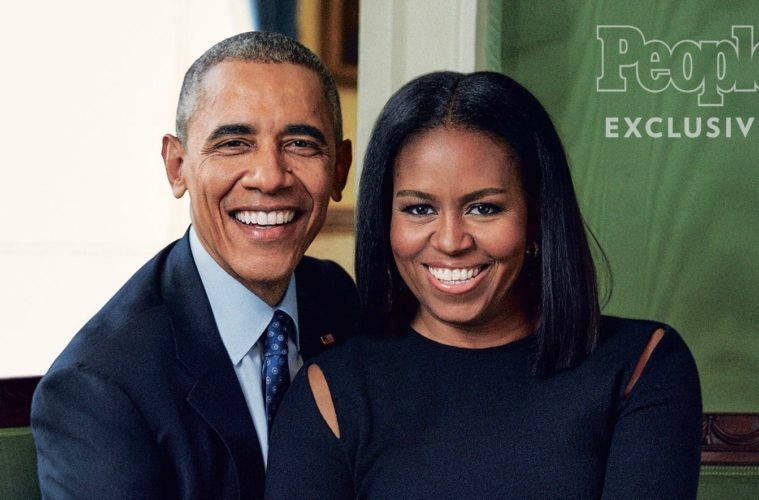
\includegraphics[scale=0.35]{images/obamas.jpg}
\end{center}
\end{frame}

\begin{frame}{Project: Facial keypoints detection}
Face detection:
\begin{center}
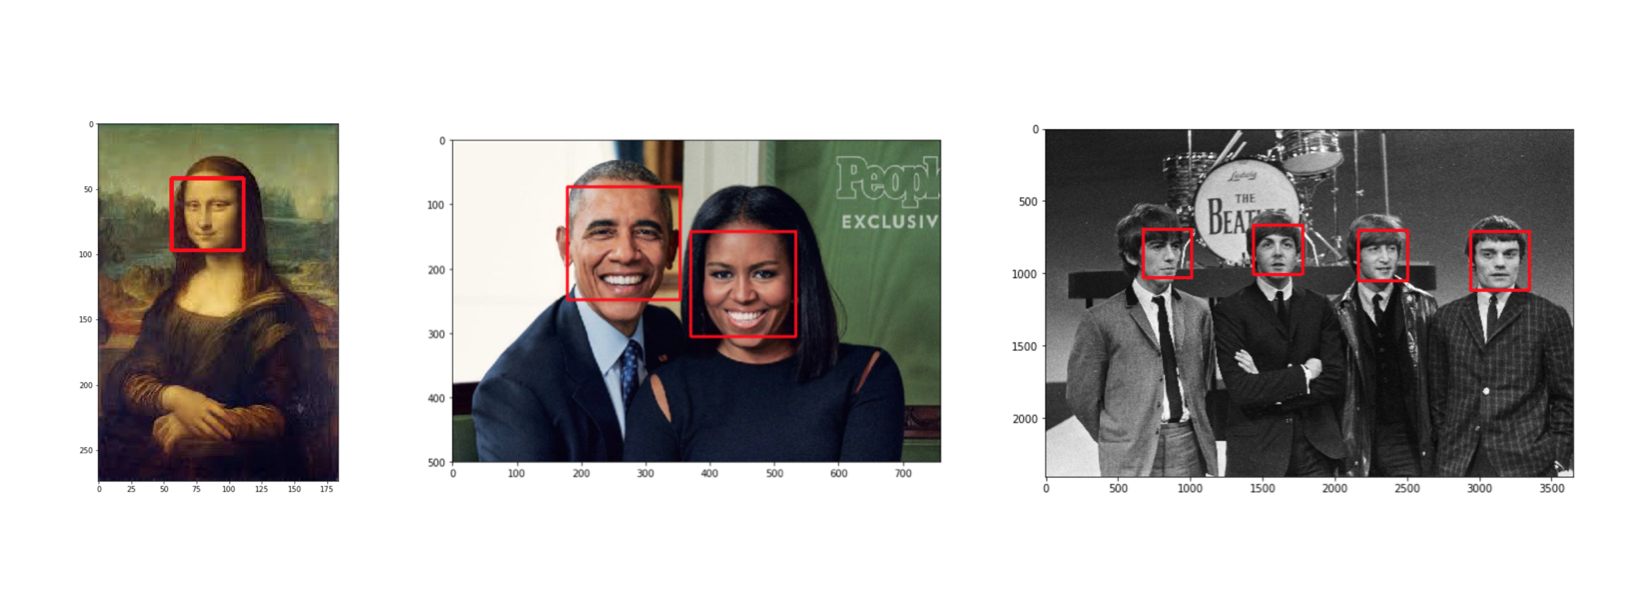
\includegraphics[scale=0.4]{images/haar_cascade_ex.png}
\end{center}
\end{frame}

\begin{frame}{Project: Facial keypoints detection}
Output:
\begin{center}
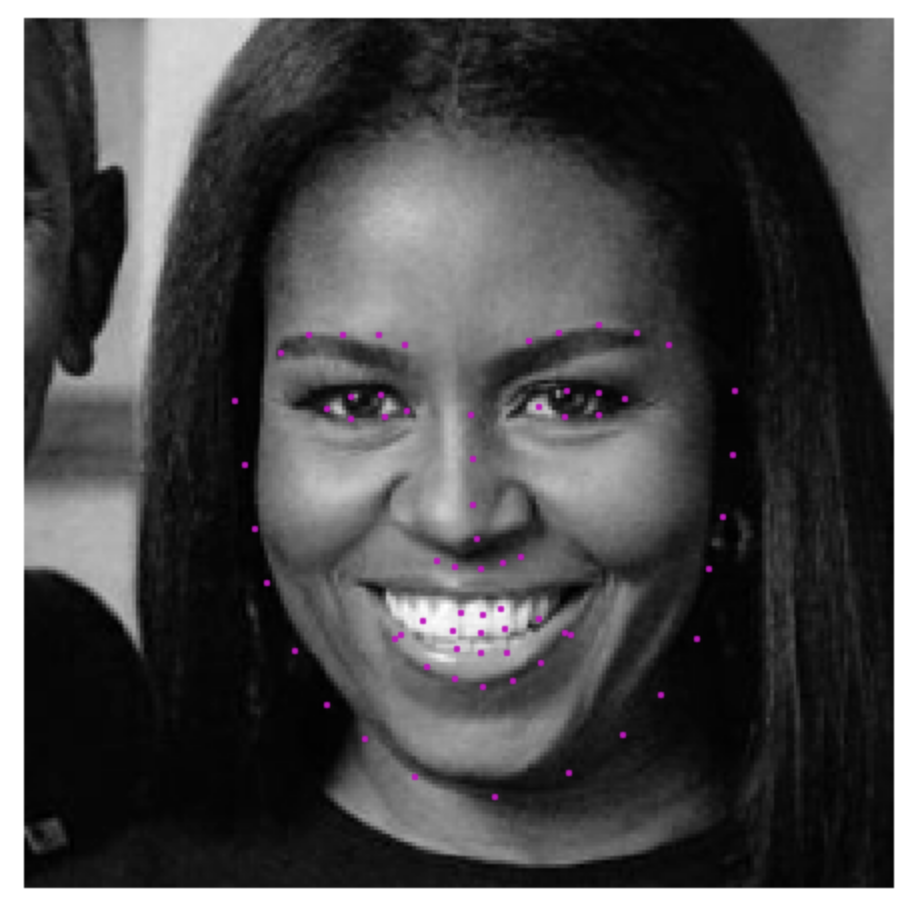
\includegraphics[scale=0.4]{images/michelle_detected.png}
\end{center}
\end{frame}

\begin{frame}{Advanced compuer vision and deep learning}
\begin{enumerate}
\item YOLO\\
You only look once: network for the real-time object detection\\
\href{https://pjreddie.com/darknet/yolo/}{Official webpage}, 
\href{https://www.youtube.com/watch?v=JLcLryo7lbQ}{Demo}

\item RNN\\
Recurrent neural network: understanding the context of the image 
\item LSTM\\
Long-short-term memory: one of the type of the RNN. This network is used to analize the context
\end{enumerate}
\end{frame}

\begin{frame}{Project: Image captioning}
Python + PyTorch + Jupyter Notebook + COCO data set + CUDA
\begin{center}
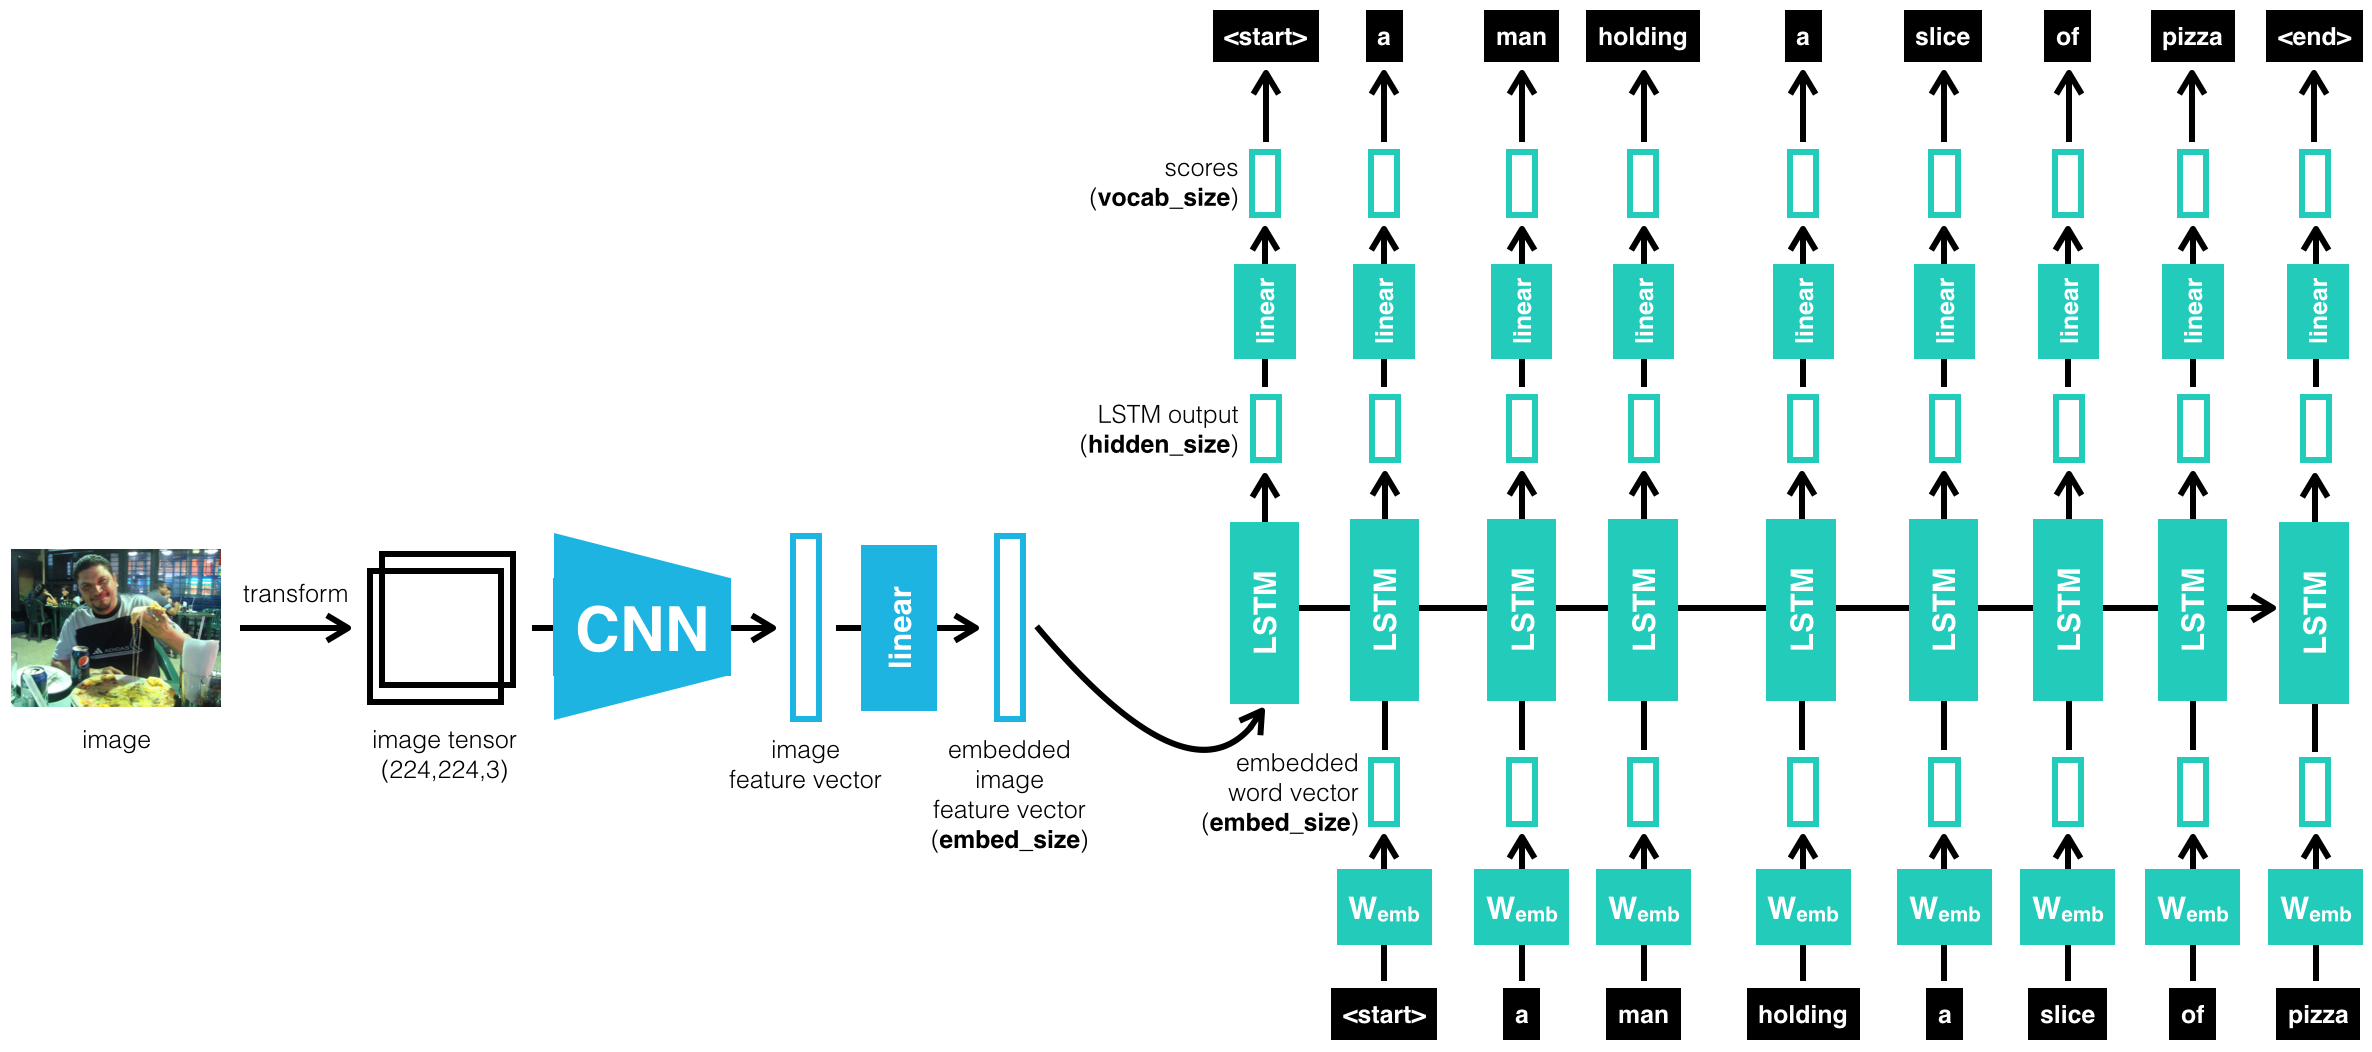
\includegraphics[scale=0.28]{images/encoder-decoder.png}
\end{center}
\end{frame}


\begin{frame}{Object tracking and lockalization}
\begin{itemize}
\item Undestanding of motion\\
Methematical representation of the motion, programm 2d map and detect objects with the motion based on the probabilities.
\item Kalman filter\\
is an algorithm that uses a series of measurements observed over time, containing statistical noise and other inaccuracies, and produces estimates of unknown variables.\\
A common application is for guidance, navigation, and control of vehicles.
\end{itemize}
\end{frame}

\begin{frame}{Project: Landmark detection and tracking (SLAM)}
Python + Jupyter notebook
\newline
\newline
Highly artificail project, that has nothing to do with the CV
\newline
\newline

The task of the project:
\begin{enumerate}
\item Programm the world, where the robot will navigate
\item Simulate each movement of the robot
\item Add some noise
\item Predict the locaion of the robot
\end{enumerate}
\end{frame}


\section{Conclusions}
\begin{frame}
\begin{center}
\Huge Conclusions
\end{center}
\end{frame}

\begin{frame}{Conclusions}
What I liked:
\begin{enumerate}
\item Was new for me to work with RNN and PyTorch.
\item Better understanding of the image pre-processing.
\end{enumerate}
\vfill
What I would change?
\begin{enumerate}
\item More teoretical stuff
\item More classic CV algorithms
\item Remove SLAM part
\end{enumerate}
\vfill
Would I recommend the nanodegree? Yes!
\vfill
Will I do another one? Yes
\vfill
If you want to do ML, DL, AI or similar, strongly recommend to have a NVidia GPU at home.
\end{frame}

\begin{frame}{Q\&A}
\begin{center}
\Huge Questions?
\end{center}
\end{frame}

\end{document}